\documentclass{beamer}

\usepackage[utf8]{inputenc}
\usepackage[T1]{fontenc}
\usepackage[french]{babel}
\usepackage[ddmmyyyy]{datetime}

\usetheme{Warsaw}
\useinnertheme{rectangles}
\setbeamerfont{headline}{size=\large}
\setbeamerfont{frametitle}{size=\normalsize}

%Plan/Sommaire automatique avant chaque section
\AtBeginSection[]{
  \begin{frame}
  \frametitle{Plan}
  \tableofcontents[currentsection]
  \end{frame}
}

\author{Sonny Klotz - Jean-Didier Pailleux - Malek Zemni}
\institute{UVSQ}
\date{\today}
\usepackage{../tex/myInfolines}
\usepackage{longtable,array}
\title{Présentation Cahier des Charges}

\begin{document}

	\begin{frame}
		\titlepage
	\end{frame}
	
	\section{Introduction}
		\begin{frame}
			Projet de L3 informatique UVSQ, remis par DCbrain.\\~\\
		\begin{itemize}
		\item Projet découlant d'un thème: le \textbf{Big Data}.
		\item Analyse descriptives de données répond au problème du \textbf{Big Data}.
		\item DCbrain emploie une approche basée sur la représentation des réseaux physiques en graphe de flux. Permet la déctection d'anomalies sur le réseau + simuler les évolutions.
		\item Objectif : Fournir application web, outils complémentaire au travail de DCbrain.
		\end{itemize}
		\end{frame}
	
	\section{Architecture}
			\begin{frame}
		\begin{center}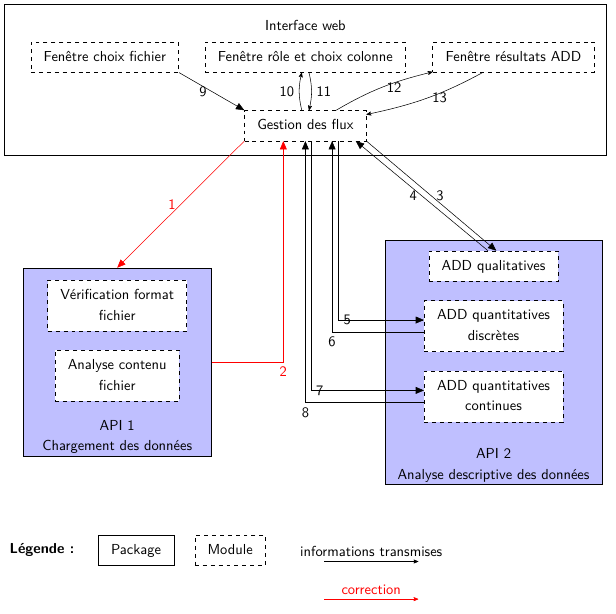
\includegraphics[scale=0.5]{org2.png}\end{center}
	\end{frame}
	
	\begin{frame}
		\textbf{API 1 :} Chargement des données\\
		\textit{Vérification format fichier :}
		\begin{itemize}
			\item Format csv
			\item Ouverture en lecture
			\item Texte brut ou formaté
		\end{itemize} \pause
		\vspace{1cm}
		\textit{Analyse contenu fichier :}
		\begin{itemize}
			\item  Lecture des données du fichier ligne par ligne + stockage de ces données dans une \textbf{structure 1} 
			\item Description des données de chaque colonne: type, nom et données erronées + stockage dans une \textbf{structure 2}.
		\end{itemize}		 		
	\end{frame}
	
	\begin{frame}
		\begin{center}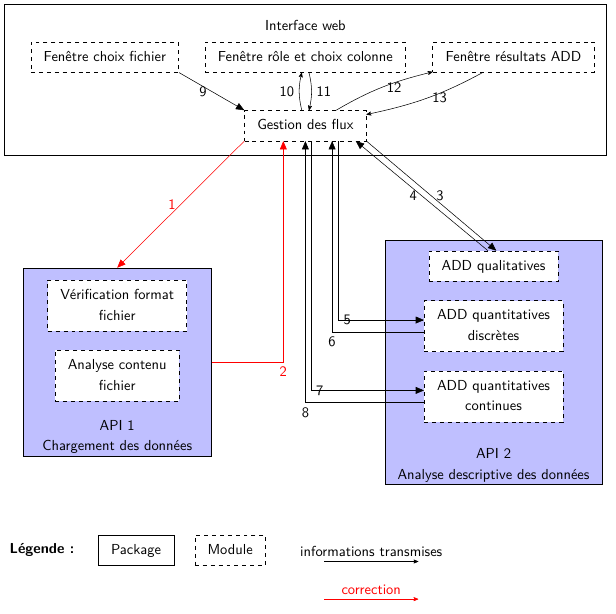
\includegraphics[scale=0.5]{org2.png}\end{center}
	\end{frame}
	
	\begin{frame}
		\textbf{API 2 :} Analyse descriptive des données\\
		\begin{itemize}
			\item \textbf{Données :} Données d'une colonne
			\item \textbf{Retour :} Informations statistiques et représentations graphiques
			\item \textbf{ADD quantitatives continues :} Discrétisation des valeurs
		\end{itemize}	
	\end{frame}
	
	\begin{frame}
		\begin{center}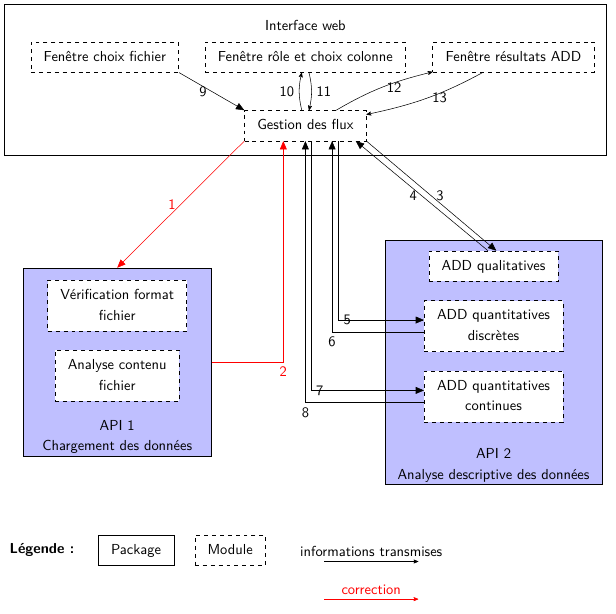
\includegraphics[scale=0.5]{org2.png}\end{center}
	\end{frame}
	
	\begin{frame}
		\textbf{Interface web}\\
		\textit{Gestion des flux :}
		\begin{itemize}
			\item Flux d'exéction : Branchements et arrêts de l'application
			\item Flux de données : Rôle d'interface pour communiquer les données
		\end{itemize} \pause
		 \vspace{1cm}
		 
		\textit{Fenêtre choix fichier :}
		\begin{itemize}
			\item Choix du fichier :Parcours de l'arborescence de fichiers - Drag \& Drop.
		\end{itemize}
	\end{frame}
	
	\begin{frame}
		\textit{Fenêtre rôle et choix colonne :}
		\begin{itemize}
		\item Nom des colonnes - Nombre de lignes et colonnes - Échantillon - Navigation.
		\item Affichage des données erronés + description.
		\item Sélection et envoi d'une colonne de mesures pour analyse. 
		\end{itemize} \pause
		 \vspace{1cm}
		 
		\textit{Fenêtre résultats ADD :}
		\begin{itemize}
		\item Affichage des résultats d'analyse descriptive : informations statistiques de l'API 2 + représentations graphiques pour visualiser les données.
		\item Fonctionnalité de retour en arrière pour analyser une nouvelle colonne.
		\item Téléchargement des résultats au format \lstinline!.csv!
		\end{itemize}
	\end{frame}
	
	\section{Outils et langages de programmation}
		\begin{frame}
			Malek (3:00)
		\end{frame}
	
	\section{Fonctionnement de l'application}
		\begin{frame}
			Malek (3:30)
		\end{frame}
	
	
	\section{Bilan technique}
		\begin{frame}
			Sonny (4:30)\\
			(3:00) : points délicats\\
			(2:00) : problèmes\\
		\end{frame}
	
	\section{Organisation interne du groupe}
		\begin{frame}
			Sonny (00:30)
		\end{frame}
	
	\section{Coûts}
		\begin{frame}
			Sonny (1:00)
		\end{frame}
	
	\section{Conclusion}
		\begin{frame}
			Sonny (1:00)
		\end{frame}
	
\end{document}
